\documentclass[12pt,a4paper,oneside,ngerman]{scrbook}

% === KONFIGURATION LADEN (richtige Reihenfolge!) ===
% ===== ENCODING UND SPRACHE =====
\usepackage[utf8]{inputenc}        % UTF-8 für Umlaute
\usepackage[T1]{fontenc}           % Bessere Fontdarstellung
\usepackage[ngerman]{babel}        % Deutsche Silbentrennung, Datumsformat

\usepackage{lmodern}               % Moderne Latin Modern Schrift
\usepackage{microtype}

% ===== SEITENLAYOUT =====
\usepackage[left=3cm,right=2.5cm,top=3cm,bottom=3cm]{geometry}
\usepackage{setspace}              % Zeilenabstand-Kontrolle
\usepackage[headsepline]{scrlayer-scrpage}  % Kopf-/Fußzeilen

% ===== MATHEMATIK UND EINHEITEN =====
\usepackage{amsmath,amssymb,amsthm}
\usepackage{mathtools}             % Erweiterte Mathe-Tools
\usepackage{siunitx}               % Korrekte Einheiten (€, m², kg, etc.)

% ===== TABELLEN =====
\usepackage{booktabs}              % Professionelle Tabellen (\toprule, \midrule, \bottomrule)
\usepackage{longtable}             % Mehrseitige Tabellen
\usepackage{array}                 % Erweiterte Tabellenfunktionen
\usepackage{multirow}              % Mehrzeilige Tabellenzellen
\usepackage{tabularx}              % Automatische Spaltenbreiten

% ===== GRAFIKEN UND ABBILDUNGEN =====
\usepackage{graphicx}              % Bilder einbinden (PDF, PNG, JPG)
\usepackage{subcaption}            % Unterabbildungen (a), (b), (c)
\usepackage{tikz}                  % Technische Zeichnungen und Diagramme
\usepackage{pgfplots}              % Professionelle Plots und Diagramme
\usepackage{xcolor}                % Farbdefinitionen

% ===== LITERATURVERZEICHNIS =====
\usepackage[
    backend=biber,
    style=authoryear-icomp,  
    maxbibnames=3,
    maxcitenames=2,
    autocite=footnote,
    date=year,
    dateuncertain=true,
    eprint=false,
    url=false,
    sorting=nyt
]{biblatex}
\addbibresource{08_bibliography/literatur.bib}
\addbibresource{08_bibliography/references.bib}

% ===== VERWEISE UND LINKS =====
\usepackage[hidelinks]{hyperref}   % Anklickbare Links (unsichtbar gedruckt)
\usepackage{cleveref}              % Intelligente Querverweise (\cref{})

% ===== LISTEN UND AUFZÄHLUNGEN =====
\usepackage{enumitem}              % Bessere Kontrolle über Listen

% ===== ANFÜHRUNGSZEICHEN UND ZITATE =====
\usepackage{csquotes}              % Korrekte deutsche Anführungszeichen

% ===== ABKÜRZUNGSVERZEICHNIS =====
\usepackage{acronym}               % Automatisches Abkürzungsverzeichnis

% ===== SPEZIELLE BAUINGENIEUR-PAKETE =====
\usepackage{textcomp}              % Zusätzliche Symbole
\usepackage{gensymb}               % Grad-Symbol und andere

\usepackage{tikz}
\usetikzlibrary{shapes.geometric, arrows.meta, positioning}

% Platzierung von Diagrammen und Tabellen
\usepackage{placeins}        % Zuerst Pakete
% ===== ZEILENABSTAND =====
\onehalfspacing                    % 1,5-facher Zeilenabstand (Standard für Masterarbeiten)

% ===== KOPF- UND FUSSZEILEN =====
\pagestyle{scrheadings}
\clearpairofpagestyles
\ohead{\headmark}                  % Kapitelname rechts oben
\ofoot{\pagemark}                  % Seitenzahl rechts unten

% ===== DEUTSCHE BESCHRIFTUNGEN FÜR QUERVERWEISE =====
\crefname{figure}{Abbildung}{Abbildungen}
\crefname{table}{Tabelle}{Tabellen}
\crefname{equation}{Gleichung}{Gleichungen}
\crefname{chapter}{Kapitel}{Kapitel}
\crefname{section}{Abschnitt}{Abschnitte}
\crefname{subsection}{Unterabschnitt}{Unterabschnitte}

% ===== EINHEITEN-KONFIGURATION (DEUTSCH) =====
\sisetup{
    locale=DE,                     % Deutsche Notation
    per-mode=fraction,             % Bruchdarstellung für Einheiten (m/s)
    output-decimal-marker={,},     % Komma statt Punkt
    group-separator={.},           % Tausender-Punkte (1.000 statt 1,000)
    group-minimum-digits=4         % Gruppierung ab 4 Stellen
}

% ===== FARBEN DEFINIEREN =====
\definecolor{tu-green}{RGB}{99,154,58}      % TU Dortmund Grün
\definecolor{tu-blue}{RGB}{0,69,136}        % TU Dortmund Blau  
\definecolor{highlight}{RGB}{220,50,50}     % Rot für Markierungen
\definecolor{gray-light}{RGB}{245,245,245}  % Hellgrau für Tabellen

% ===== GRAFIK-EINSTELLUNGEN =====
\graphicspath{{05_figures/}}                % Standardpfad für alle Bilder

% ===== TIKZ/PGFPLOTS KONFIGURATION =====
\usetikzlibrary{positioning,shapes,arrows,calc}
\pgfplotsset{compat=1.18}

% Standardfarben für Diagramme
\pgfplotscreateplotcyclelist{tu-colors}{
    {tu-green, mark=*},
    {tu-blue, mark=square*},
    {highlight, mark=triangle*},
}

% ===== TABELLEN-STYLING =====
% Professionelle Tabellen mit booktabs
\setlength{\heavyrulewidth}{1.2pt}
\setlength{\lightrulewidth}{0.6pt}

% ===== LISTEN-KONFIGURATION =====
\setlist[itemize]{nosep, left=0pt}          % Kompakte Aufzählungen
\setlist[enumerate]{nosep, left=0pt}        % Kompakte Nummerierungen

% ===== ABKÜRZUNGSVERZEICHNIS-STIL =====
\renewcommand*{\acsfont}[1]{\textsc{#1}}    % Abkürzungen in Kapitälchen

% ===== ZUSÄTZLICHE HYPERLINK-EINSTELLUNGEN =====
% (Grundeinstellungen bereits in packages.tex definiert)
\hypersetup{
    bookmarksnumbered=true,        % Nummerierte Bookmarks im PDF
    bookmarksopen=true,            % Bookmarks aufgeklappt
    pdfstartview=FitH             % PDF startet mit Seitenbreite
}

% ===== QUELLENANGABEN KONFIGURATION =====
% Anpassungen für deutsches Literaturverzeichnis
\DefineBibliographyStrings{ngerman}{
    andothers = {et\,al\adddot},
    pages = {S\adddot},
    page = {S\adddot}
}

% ===== CAPTION-STYLING =====
\captionsetup{
    format=plain,
    font=small,
    labelfont=bf,
    textfont=it,
    justification=centering,
    singlelinecheck=false
}

% ===== ZUSÄTZLICHE ABSTÄNDE =====
\setlength{\parindent}{0pt}        % Keine Einrückung bei Absätzen
\setlength{\parskip}{6pt}          % Abstand zwischen Absätzen        % Dann Einstellungen  
\title{Target Value Design im Bauwesen -- Strukturierte Analyse und prozessorientierte Darstellung im Kontext der deutschen Baupraxis}
\author{Lasse Krisztian}
\date{\today}

% ===== PERSÖNLICHE DATEN =====
\newcommand{\matrikelnummer}{184406}
\newcommand{\emailadresse}{lasse.krisztian@tu-dortmund.de}

% ===== UNIVERSITÄTSDATEN =====
\newcommand{\universitaet}{Technische Universität Dortmund}
\newcommand{\fakultaet}{Fakultät für Architektur und Bauingenieurwesen}
\newcommand{\lehrstuhl}{Lehrstuhl für Baubetrieb und Bauprozessmanagement}
\newcommand{\studiengang}{Bauingenieurwesen Vertiefung Baubetrieb}
\newcommand{\abschluss}{Master of Science (M.Sc.)}

% ===== BETREUUNG =====
\newcommand{\professor}{Univ.-Prof. Dr.-Ing. Mike Gralla}
\newcommand{\erstbetreuer}{Franziska Blennemann, M.Sc.}
\newcommand{\zweitbetreuer}{Dipl.-Ing. Tim Brandt}

% ===== TERMINE =====
\newcommand{\abgabedatum}{15. Dezember 2025}
\newcommand{\bearbeitungszeitraum}{Juli 2025 -- Dezember 2025}

% ===== THEMA UND SCHWERPUNKTE =====
\newcommand{\themabereich}{Target Value Design}
\newcommand{\untertitel}{Eine Analyse moderner Kostensteuerungsmethoden im Bauwesen}
\newcommand{\schlagwoerter}{Target Value Design, Lean Construction, Integrated Project Delivery, Bauwirtschaft}

% ===== PDF-METADATEN =====
\hypersetup{
    pdftitle={Target Value Design im Bauingenieurwesen},
    pdfauthor={Lasse Krisztian},
    pdfsubject={Masterarbeit Bauingenieurwesen},
    pdfkeywords={Target Value Design, Lean Construction, Bauwirtschaft, IPD},
    pdfcreator={LaTeX with Overleaf},
    pdfproducer={LaTeX}
}        % Zuletzt Metadaten

\begin{document}

\begin{titlepage}
    \centering
    
    % === UNIVERSITÄTS-LOGO UND NAME (oben) ===
    \vspace*{1cm}
    
    % TU Dortmund Logo
    
\includegraphics[width=0.3\textwidth]{tud_logo_cmyk}\\[0.5cm]
    
    {\Large \textbf{\universitaet}}\\[0.3cm]
    {\large \fakultaet}\\[0.2cm]
    {\normalsize \lehrstuhl}\\[2cm]
    
    % === TITEL DER ARBEIT ===
    {\huge \textbf{\@title}}\\[1.5cm]
    
    % === ART DER ARBEIT ===
    {\Large Masterarbeit}\\[0.3cm]
    {\large zur Erlangung des akademischen Grades}\\[0.2cm]
    {\large \textbf{\abschluss}}\\[0.2cm]
    {\normalsize im Studiengang \textbf{\studiengang}}\\[2cm]
    
    % === VERFASSER ===
    \begin{tabular}{ll}
        \textbf{Verfasser:} & \@author \\[0.2cm]
        \textbf{Matrikelnummer:} & \matrikelnummer \\[0.2cm]
        \textbf{E-Mail:} & \emailadresse \\[1cm]
    \end{tabular}\\[1.5cm]
    
    % === BETREUUNG ===
    \begin{tabular}{ll}
        \textbf{Erstprüfer:} & \professor \\[0.2cm]
        \textbf{Erstbetreuer:} & \erstbetreuer \\[0.2cm]
        \textbf{Zweitbetreuer:} & \zweitbetreuer \\[1cm]
    \end{tabular}\\[1cm]
    
    % === TERMINE ===
    \begin{tabular}{ll}
        \textbf{Bearbeitungszeitraum:} & \bearbeitungszeitraum \\[0.2cm]
        \textbf{Abgabedatum:} & \abgabedatum \\
    \end{tabular}
    
    \vfill
    
    % === DATUM (unten) ===
    {\normalsize Dortmund, \abgabejahr}
    
\end{titlepage}

% Leere Rückseite für doppelseitigen Druck
\thispagestyle{empty}
\cleardoublepage
\cleardoublepage
\phantomsection
\chapter*{Abstract}
\markright{Abstract} % Setzt die Kopfzeile

“Target Value Design in Construction: A Structured and Process-Oriented Analysis within the German Context.”
\cleardoublepage
\chapter*{Vorwort}
\markright{Vorwort}

% === VORSPANN (römische Seitenzahlen) ===
\frontmatter
\tableofcontents
\chapter{Abkürzungsverzeichnis}
\markright{Abkürzungsverzeichnis}

% Short-first nur bei der ersten Stelle; danach gilt "benutzt".
\newcommand{\acsf}[1]{\acs{#1} (\acl{#1})\acused{#1}}

\begin{acronym}[PRISMA]  % Längste Abkürzung für Spaltenbreite
    \acro{AHO}{Ausschuss der Verbände und Kammern der Ingenieure und Architekten für die Honorarordnung}
    \acro{BIM}{Building Information Modeling}
    \acro{IPA}{Integrierte Projektabwicklung}
    \acro{IPD}{Integrated Project Delivery}
    \acro{LC}{Lean Construction}
    \acro{HOAI}{Honorarordnung für Architekten und Ingenieure}
    \acro{PRISMA}{Preferred Reporting Items for Systematic Reviews and Meta-Analyses}
    \acro{TVD}{Target Value Design}
    \acro{VOB}{Vergabe- und Vertragsordnung für Bauleistungen}
\end{acronym}
\listoffigures
\listoftables


% === HAUPTTEIL (arabische Seitenzahlen) ===
\mainmatter
\chapter{Einleitung (Exposé)}
\label{ch:einleitung}

\section*{Problemstellung und Relevanz}
\label{sec:problemstellung}
Die deutsche Bau-- und Infrastrukturbranche steht vor immensen Herausforderungen, die  eine grundlegende Steigerung der Effizienz und Umsetzungsgeschwindigkeit erfordern.  Ein signifikantes Wohnungsbaudefizit, das je nach Studie auf über 550.000 fehlende  Wohnungen beziffert wird, verlangt nach einer drastischen Beschleunigung des Neubaus\autocite[]{}. Gleichzeitig stellt die  Bundesregierung über ein neues Sondervermögen für Infrastruktur und Klimaschutz bis  2029 mehr als 100 Milliarden Euro an Mitteln jeweils für den Bahn- und Wohnungsbau  bereit\autocite[]{brinkmeier2025}. Die Umsetzung der bereitgestellten Mittel in den dringend  benötigten Projekten droht jedoch an strukturellen Problemen wie dem eklatanten  Fachkräftemangel, anhaltenden Kapazitätsengpässen in der Bauwirtschaft und  langwierigen Genehmigungsverfahren zu scheitern\autocite[]{hdb2025}.

\begin{figure}[htbp]
    \centering
    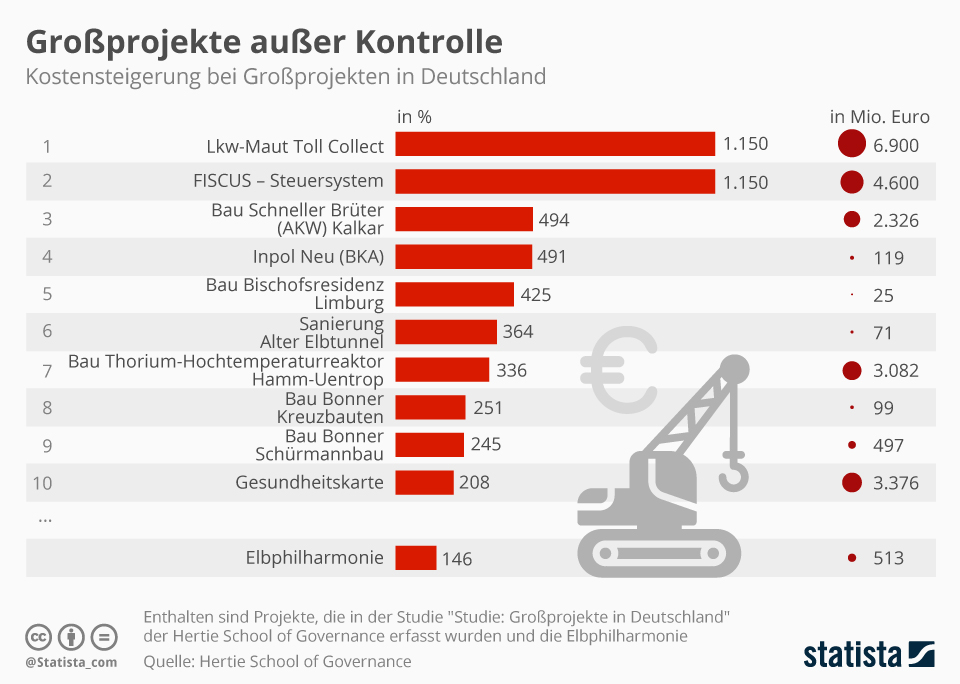
\includegraphics[width=0.9\textwidth]{kostensteigerung-grossprojekte-deutschland}
    \caption{Kostensteigerungen bei deutschen Großprojekten \cite{statista2024grossprojekte}}
    \label{fig:kostensteigerung-grossprojekte}
\end{figure}
\clearpage
Zusätzlich steht diese Bedarfslage einer traditionell fragmentierten und sequentiell  organisierten Projektabwicklung gegenüber. Die etablierte Projektkultur, die stärker auf  vertragliche Abgrenzung als auf Zusammenarbeit ausgerichtet ist, begünstigt strukturelle  Ineffizienzen sowie Kosten-- und Terminüberschreitungen, die bei öffentlichen  Großprojekten im Durchschnitt bei über 40\% liegen\autocite[]{korn2019}. Vor dem  Hintergrund der aktuellen Herausforderungen erscheinen diese Eigenschaften  zunehmend problematisch.

Ein vielversprechender Lösungsansatz, welcher sich international bereits etabliert hat,  bieten integrierte Projektabwicklungsmodelle wie das Project Alliancing oder die  Integrierte Projektabwicklung (IPA). Bei diesen Arten der Projektabwicklung liegt der  Fokus auf einem kollaborativen, gemeinschaftlichen Ansatz, bei dem die wesentlichen  Akteure frühzeitig in einem Mehrparteienvertrag gebunden werden, um Risiken und  Chancen gemeinsam zu managen und das Projekt auf den Gesamterfolg auszurichten.  Dieser Ansatz hat sich international als äußerst erfolgreich bei der Realisierung  komplexer Vorhaben bewährt\autocite[]{cook2014}.

In den letzten Jahren hat das IPA--Thema auch in Deutschland stark an Fahrt aufgenommen und findet derzeit in mehr und mehr Pilotprojekten Anwendung. Das IPA--Zentrum identifizierte in seinem Jahresbericht von 2024 insgesamt 25 abgeschlossene oder laufende IPA--Projekte und weitere, bei denen eine aktive Entscheidung für IPA bereits gefallen ist (vgl. Haghsheno et al 2024). Ein zentraler Prozessbaustein zur Kosten-- und Wertsteuerung innerhalb dieser Modelle ist das Target Value Design (TVD)\autocite[]{Testkey}. Während zu den übergeordneten IPA--Rahmenbedingungen bereits Forschung im deutschen Kontext existiert\autocite[]{haghsheno2024}, fehlt eine systematische, prozessorientierte  Aufbereitung für die Anwendung von TVD (siehe Kapitel 3). Hier setzt die vorliegende  Arbeit an, um diese Lücke zu schließen und aufzuzeigen, wie TVD als Methode zur Bewältigung der anstehenden Bauaufgaben beitragen kann.

\section*{Zielsetzung und Forschungsfrage}
\label{sec:zielsetzung}

\subsection*{Hauptziel und zentrale Forschungsfrage}
Das Hauptziel dieser Arbeit besteht in der systematischen Analyse und Aufbereitung des Target Value Design (TVD) als zentraler Bestandteil moderner, integrierter Projektabwicklungsmodelle im Bauwesen wie der Integrierten Projektabwicklung (IPA). Dabei sollen, anhand einer systematischen Literaturrecherche, wesentliche Prozessbausteine des TVD identifiziert und beschrieben werden, um sie anschließend zu einem idealtypischen Gesamtprozess zusammenzusetzen. Die tiefgehende Aufbereitung und Darstellung sollen im Anschluss eine optimale Gegenüberstellung mit den Abläufen der konventionellen Projektabwicklung in Deutschland ermöglichen. Dieser Vergleich konzentriert sich insbesondere auf die Rahmenbedingungen in der deutschen Baupraxis, die von den einschlägigen Regelwerken wie HOAI und AHO geschaffen werden, und dient vor allem der Identifizierung von Anpassungsbedarfen. Letztere sollen schlussendlich in der Ableitung eines Transferleitfadens münden, der die Anwendung von TVD im Kontext der Bauprojektabwicklung in Deutschland verbessert.

Daraus leitet sich die folgende zentrale Forschungsfrage ab:

\enquote{Wie lässt sich der Target Value Design-Prozess strukturiert in Einzelschritte zerlegen, nachvollziehbar darstellen und für die Anwendung in der deutschen Baupraxis übersetzen, um den strukturellen Defiziten der traditionellen Projektabwicklung entgegenzuwirken?}

\subsection*{Exploratives Nebenziel}
Ergänzend zum Hauptziel soll diese Arbeit einen explorativen Ausblick auf eine weitere Forschungslücke, die mögliche Übertragbarkeit von TVD im Hochbau auf Infrastrukturprojekte \autocite [S.45]{ballard2025}, gewähren. Ziel ist es aufzuzeigen, welche spezifischen Charakteristika diese Bauprojektarten (z.\,B. Linienbaustellen) aufweisen und welche der zuvor herausgearbeiteten Bausteine des TVD hier potenziell anwendbar wären bzw. einer Anpassung bedürfen.

\subsection*{Hypothese und erwartete Erkenntnisse}
Die zentrale Hypothese dieser Arbeit lautet, dass eine direkte Übertragung des TVD-Prozesses auf die deutsche Baupraxis aufgrund der strukturellen, rechtlichen und kulturellen Rahmenbedingungen nicht zielführend ist. Vielmehr wird angenommen, dass eine erfolgreiche Implementierung von Target Value Design über die bloße Einführung einer Methode hinausgeht und spezifische Anpassungen erfordert, um den Gegebenheiten in Deutschland gerecht zu werden.
Als Ergebnis dieser Arbeit soll ein Transferleitfaden für die Anwendung von Target Value Design in Deutschland entstehen. Dieser Leitfaden soll sowohl den aufbereiteten Prozess darstellen als auch Inkompatibilitäten aufzeigen und konkrete Handlungsempfehlungen für letztere bieten, um eine effiziente Projektabwicklung mit Target Value Design zu ermöglichen.

\section*{Methodischer Ansatz}
\label{sec:methodischer-ansatz}

Die Arbeit verfolgt einen literaturbasierten, konzeptionell-analytischen Forschungsansatz, der sich in drei aufeinander aufbauende Schritte gliedert:

\begin{enumerate}
    \item \textbf{Systematische Literaturrecherche und -analyse:} Zunächst werden die theoretischen Grundlagen durch eine systematische Literaturrecherche erarbeitet. Dabei werden einschlägige wissenschaftliche Datenbanken (z.\,B. Scopus, Web of Science) sowie relevante Publikationen von Fachinstitutionen (z.\,B. LCI, GLCI, IPA-Zentrum) ausgewertet. Die Recherche wird durch gezielte Suchstrategien (Keyword Kombinationen) und Auswahlkriterien (z.\,B. Aktualität, Relevanz) strukturiert, um internationale Standardwerke zu TVD und IPA sowie Fachliteratur zu den spezifischen Rahmenbedingungen der deutschen Baupraxis zu identifizieren und zu analysieren.
    
    \item \textbf{Prozessbeschreibung und Modellierung:} Auf Basis der analysierten Literatur wird ein idealtypisches Prozessmodell des TVD konstruiert. Dieses Modell zerlegt den Gesamtprozess in seine wesentlichen Phasen, Rollen, Entscheidungspunkte und Abhängigkeiten und visualisiert deren Zusammenspiel.
    
    \item \textbf{Kontextanalyse und Ableitung des Transferleitfadens:} Das idealtypische TVD-Modell wird anschließend den strukturellen, technischen, rechtlichen und kulturellen Gegebenheiten der deutschen Baupraxis im Hochbau gegenübergestellt. Aus dieser Gegenüberstellung werden Reibungspunkte und Anpassungsbedarfe identifiziert. Die Ergebnisse münden in der Entwicklung eines konzeptionellen Transferleitfadens, der konkrete Handlungsempfehlungen für die Anwendung von TVD in Deutschland formuliert.
\end{enumerate}

Für das explorative Nebenziel der Übertragbarkeit von TVD auf Infrastrukturprojekte werden die aus dem Hochbau gewonnenen Erkenntnisse auf die spezifischen Charakteristika dieser Projektart angewandt, um erste Hypothesen für notwendige Adaptionen aufzuzeigen.

\section*{Aufbau der Arbeit}
\label{sec:aufbau}

\chapter{Grundlagen}
\label{ch:grundlagen}


\section{Konventionelle Projektabwicklung in der deutschen Baupraxis}
\label{sec: 2.1}
Ziel: Der Leser soll die Struktur, die Rollenverteilung und die prozessualen Schwachstellen der traditionellen Projektabwicklung verstehen. Dieses Kapitel etabliert das "Problem", für das die Arbeit eine Lösung präsentiert.

\subsection{Einleitung -- Die etablierte Ordnung}
\label{sec: 2.1.1}
Zielsetzung: Den Leser in das Thema einführen und die prägenden Regelwerke der konventionellen Projektabwicklung in Deutschland benennen.\\
- Feststellung: Die deutsche Baupraxis wird maßgeblich durch HOAI und VOB geformt.\\
- Grundprinzip herausarbeiten: Strikte Trennung von Planungs- und Ausführungsleistungen.\\
- Charakterisierung des Modells: Sequenzieller Ablauf in Phasen.\\



\subsection{Das Prozessmodell - HOAI Leistungsphasen}
\label{sec: 2.1.2}
Zielsetzung: Das abstrakte "Phasenmodell" mit dem konkreten Ablauf der HOAI-Leistungsphasen füllen und dessen starre, lineare Struktur verdeutlichen.\\
- Prozessstruktur: Wird durch die neun Leistungsphasen der HOAI definiert.\\
- Darstellung des Ablaufs: Inhärent linear und sequenziell (LPH 1 -> LPH 9).\\
- Kritischen Punkt identifizieren: Wesentliche Kosten- und Qualitätsentscheidungen fallen in den frühen Planungsphasen (insb. LPH 2-3).\\
- Problem benennen: Zu diesem frühen Zeitpunkt fehlt die vertraglich gebundene Expertise der Ausführung.\\
- Empfehlung: Visualisierung des linearen Ablaufs durch ein einfaches Diagramm.\\

\subsection{Die Organisationsstruktur - getrennte Silos}
\label{sec: 2.1.3}
Zielsetzung: Die prozessuale Trennung auf die organisatorische Ebene übertragen und das Problem der isolierten Akteure (Silos) einführen.\\
- Organisationsstruktur beschreiben: Klassische Dreieckskonstellation (Bauherr, Planer, Ausführender) mit bilateralen Verträgen.\\
- Problem der "Silos" formulieren: Jeder Akteur ist primär auf die Erfüllung des eigenen Vertrags fokussiert.\\
- Kommunikationswege: Oft nur indirekt über den Bauherrn, nicht disziplinübergreifend.\\

\subsection{Die Konsequenzen - strukturelle Schwachstellen}
\label{sec: 2.1.4}
Zielsetzung: Die negativen, systemischen Folgen der beschriebenen Struktur klar benennen und mit Belegen untermauern. Dies ist der Kern der Problemanalyse.\\
- Schwachstellen auflisten und erläutern:\\
- Späte Einbindung von ausführendem Know-how.\\
- Informationsverluste an den Schnittstellen.\\
- Entstehung eines adversialen Projektklimas (Fokus auf Nachtragsmanagement).\\
- Direkte Verbindung zu Kosten- und Terminüberschreitungen herstellen\\

\subsection{Fazit und Überleitung}
\label{sec: 2.1.5}
Zielsetzung: Den Abschnitt abschließen und eine Brücke zum folgenden Kapitel schlagen.\\

- Zusammenfassen: Das konventionelle Modell bietet zwar einen klaren rechtlichen Rahmen, weist jedoch inhärente Schwächen auf, die Effizienz und Kooperation behindern.
- Schlussfolgerung: Angesichts aktueller Herausforderungen ist das Modell zunehmend reformbedürftig.\\
- Überleitung formulieren: Hinweis auf die Entwicklung alternativer, international etablierter Projektabwicklungsmodelle als Reaktion auf diese Defizite.

\clearpage

\section{Integrierte Projektabwicklungsmodelle als alternativer Ansatz}
\label{sec: 2.2}

% Ziel: Der Leser soll eine Einführung in die Entstehung und Entwicklung integrierter Projekabwicklung bekommen.

\subsection{Der Lean-Ansatz als Fundament der \ac{IPA}}
\label{sec:2.2.1}

% Ziel: Vermittlung der Lean-Pilosophie als Ursprungsgedanke und der Weiterentwicklung über Lean Construction zu kollaborativen Projekabwicklungsmodellen

Die im vorangegangenen Abschnitt aufgezeigten Schwachstellen konventioneller, sequenzieller Projektabwicklung sind keineswegs ein neues Phänomen oder eine reine Eigenheit der Bauwirtschaft. Vergleichbare Herausforderungen zeigten sich bereits nach dem Zweiten Weltkrieg in der japanischen Automobilindustrie. Die dort vorherrschenden Produktionsmethoden waren von Ineffizienz und Verschwendung geprägt, was angesichts knapper Ressourcen nicht tragbar war. Als Reaktion darauf entwickelte der Ingenieur Taiichi Ohno bei Toyota einen grundlegend neuen Managementansatz, der heute als das Toyota-Produktionssystem bekannt ist und das Fundament der Lean-Philosophie bildet.

Ursprung des Ansatzes (Lean Management) Skizzieren
- Toyota-Produktionssystem\autocite[]{ohno_toyota-produktionssystem_2013} als Ursprung
- Kernideen und Prinzipien : Wertmaximierung, Verschwendungsreduktion, People First (checken), Kaizen

Transfer auf die Baubranche durch Lean Construction
- Landesweite Aufmerksamkeit in Japan nach der Ölkrise 1973
- Während sich die 
- Internationale Aufmerksamkeit durch 

Ursprung und Entwicklung von Projetct Alliancing, IPD und IPA bis heute

\subsection{Prinzipien und Merkmale der Integrierten Projektabwicklung (IPA)}
\label{sec:2.2.2}

IPA als ist das organisatorische und vertragliche "Betriebssystem", um die Lean-Philosophie in Bauprojekten praktisch umzusetzen.\\

Schlüsseleigenschaften und IPA-Charakteristika:\\
- Frühzeitige Integration aller Schlüsselpartner (Planer und Ausführende) von Beginn an.\\
Ein Mehrparteienvertrag, der alle Partner an einen Tisch bindet.\\
Ein gemeinsames Risikomanagement (Chancen-/Risikopool).\\
Eine kollaborative Kultur und gemeinsame Entscheidungsfindung.\\


\subsection{Internationale Erfolge und Status Quo in Deutschland}
\label{sec:2.2.3}



International: Hohe Erfolgsquoten im angelsächsischen Raum (USA, UK, Australien mit "Project Alliancing") bei der Einhaltung von Kosten und Terminen (Quelle z.B. cook2014).\\

Deutschland: Das Thema gewinnt stark an Fahrt: es gibt eine wachsende Zahl an Pilotprojekten (Quelle: IPA-Report 2024 von haghsheno2025).\\

Eine zentrale Kernmethode zur Kosten- und Wertsteuerung innerhalb dieser IPA-Modelle ist das Target Value Design.\\
\clearpage

\section{Target Value Design (TVD) als Kernmethode}
\label{sec: 2.3}

%Ziel:

\subsection{TVD - Prozess oder Methode}
\label{sec: 2.3.1}

% =======================================================
% FÜR ABSCHNITT 2.3.1: TVD - Prozess oder Methode
% =======================================================
%https://service.tu-dortmund.de/group/intra/ausstattung-lokaler-arbeitsplatze
%   - Ziel: Eine präzise und trennscharfe Definition von TVD für die
%     vorliegende Arbeit herleiten. Es soll geklärt werden, ob TVD als
%     Prozess, als Methode oder als beides zu verstehen ist, um eine
%     eindeutige Basis für die nachfolgende Analyse zu schaffen.
%
%   - Einstieg: Feststellung, dass die Begriffe "Prozess" und "Methode"
%     in der Literatur zu TVD oft unscharf oder synonym verwendet werden.
%
%   - Begriffsdefinition "Methode": Ein systematisches, geplantes Vorgehen,
%     das auf Prinzipien, Regeln und Werkzeugen basiert, um ein Ziel zu erreichen.
%
%   - Begriffsdefinition "Prozess": Eine logische und zeitliche Abfolge von
%     miteinander verknüpften Aktivitäten zur Umwandlung eines Inputs in einen Output.
%
%   - Anwendung auf TVD:
%     - TVD ist mehr als ein reiner Prozess, da es eine bestimmte Denkweise
%       ("Target First"), Prinzipien (Kollaboration) und Werkzeuge voraussetzt.
%     - Diese übergeordnete Denkweise wird jedoch erst durch einen konkreten,
%       strukturierten Ablauf (Prozess) in der Praxis anwendbar.
%
%   - Fazit & Positionierung: Für diese Arbeit wird TVD als eine
%     *MANAGEMENT-METHODE* verstanden, die durch einen
%     _STRUKTURIERTEN PROZESS_ operationalisiert und umgesetzt wird.
%     Diese Definition legitimiert die nachfolgende "prozessorientierte
%     Darstellung" der Methode.
%
% =======================================================

Zur Hinleitung auf die in \cref{ch:methodik} beschriebene, methodische Vorgehensweise soll an dieser Stelle auf das in dieser Arbeit zu Grunde liegende Verständnis von \ac{TVD} als Prozess bzw. Methode eingegangen werden.\\
In der Literatur ist die Abgrenzung zwischen Prozess und Methode in der aktuellen Diskussion um TVD unscharf. Folgt man dem Ergebnis einer einfachen Stichwortsuche in einschlägigen wissenschaftlichen Datenbanken (z.B. reseachgate.net) so wird schnell deutlich, das in der überwiegenden Mehrheit der Literatur (ca. 70\%) Target Value Design als Prozess verstanden wird.
Glenn Ballard, der als einer Gründer des \ac{TVD} gilt, bezeichnet letzteres hingegen häufig als Managementansatz bzw. Management-Methode \autocite[]{}.\\
% In der allgemeinen Literatur wird ein Prozess als

- Definition Prozess Vs. Methode: Verständnis als Management Methode die durch einen sturkturierten Prozess umgesetzt wird -> legitimiert die nachfolgende prozessoroentierte Darstelung.\\

\subsection{Ziele und Grundprinzipien von TVD}
\label{sec: 2.3.2}

Ziel: Kosten als Inputgröße statt Outputgröße der Planung.\\

Prinzipien:\\
- Set-based Design\\
- Collaborative Cost Estimation\\
- Value Definition durch den Nutzer\\
- Continuous Cost Validation\\
- ggf. Bezug zu Lean-Grundsätzen (Wert, Fluss, Pull, Perfektion).\\

\subsection{Prozessstruktur und Rollen im TVD-Prozess}
\label{sec: 2.3.3}

- Phasenstruktur nach Literatur\\
- Rollen und Verantwortlichkeiten\\
- Kommunikations- und Entscheidungslogik\\
- Fazit / Relevanz für die Arbeit\\

\subsection{Abgrenzung und Schnittstellen zu verwandten Methoden}
\label{sec: 2.3.4}

- Unterschied zu Target Costing (Industrie) und Value Engineering (klassische Planung).\\

- Einordnung in IPA-Kontext.\\

- Relevanz: Warum TVD nicht nur Kostentechnik, sondern Führungsprinzip ist.\\

\subsection{Fazit und Überleitung zur Methodik}
\label{sec: 2.3.5}
- TVD als prozessorientierte Managementmethode mit systematischer Kosten- und Wertsteuerung.\\

Zur detaillierten Untersuchung dieses Prozesses im Kontext der deutschen Baupraxis wird im folgenden Kapitel das methodische Vorgehen beschrieben. Dabei wird zunächst das Forschungsdesign erläutert und anschließend dargelegt, wie der idealtypische TVD-Prozess systematisch analysiert und modelliert wird.

\clearpage
\chapter{Methodik}
\label{ch:methodik}

% Ziel: Das Vorgehen der Arbeit transparent und wissenschaftlich nachvollziehbar darlegen.
% Es wird der "Plan" für die Forschung beschrieben.

Wie in \cref{ch:einleitung} dargelegt, erfordert die Bewältigung der aktuellen Herausforderungen im Bauwesen neue Ansätze der Projektabwicklung wie \

\section{Forschungsdesign und methodische Verortung}
\label{sec: 3.1}
%   - Ziel: Wahl der Methodik begründen und wissenschaftlich einordnen.
%   - Inhalt:
%     - Wiederholung der Forschungsfrage.
%     - Begründung für literaturbasierten, konzeptionell-analytischen Ansatz.
%     - Abgrenzung zu anderen Methoden (z.B. empirisch).
%     - Optional: Visualisierung des Vorgehens als einfaches Flussdiagramm.
\subsection{Herleitung des Forschungsbedarfs aus der Forschungsfrage}
\label{sec: 3.1.1}

%   Wiederholung der Forschungsfrage prägnant
%   Ableitung der notwendingen Schritte zur Beantwortung
%   


\subsection{Einordnung in das Forschungsparadigma: Ein qualitativ-konstruktiver Ansatz}
\label{sec: 3.1.2}

\subsection{Wahl des konkreten Forschungsdesigns: Die konzeptionell-analytische Arbeit}
\label{sec: 3.1.3}

  \subsection{Gütekriterien des qualitativen Forschungsdesigns}
\label{sec: 3.1.4}

\subsection{Visualisierung des Forschungsprozesses}
\label{sec: 3.1.5}

% Definition von Stilen, um den Code sauber zu halten
\tikzset{
  phase/.style={rectangle, rounded corners, draw=black, fill=gray!10,
                text width=0.85\textwidth, minimum height=1.5cm, text centered},
  pfeil/.style={-latex, thick}
}

\begin{figure}[hbt!]
  \makebox[\textwidth][c]{
    \begin{tikzpicture}
      \tikzset{
        phase/.style={rectangle, rounded corners, draw=black, fill=gray!10,
                      text width=0.9\textwidth, minimum height=1.5cm, text centered},
        pfeil/.style={-latex, thick}
      }

      \node[phase] (phase1) {
        \textbf{Phase 1: Forschungsdesign (Kap. 3.1)}\\
        \small Problemstellung, Methodische Verortung, Konzeptionell-analytischer Ansatz
      };

      \node[phase, below=0.8cm of phase1] (phase2) {
        \textbf{Phase 2: Literaturanalyse (Kap. 3.2)}\\
        \small Systematische Recherche, Qualitative Inhaltsanalyse, Identifikation von Bausteinen
      };

      \node[phase, below=0.8cm of phase2] (phase3) {
        \textbf{Phase 3: Modellkonstruktion (Kap. 3.3)}\\
        \small Synthese der Bausteine, Modellierung des idealtypischen TVD-Prozesses
      };

      \node[phase, below=0.8cm of phase3] (phase4) {
        \textbf{Phase 4: Kontextanalyse \& Transfer (Kap. 3.4)}\\
        \small Fit-Gap-Analyse (Vergleich mit HOAI/VOB), Ableitung des Transferleitfadens
      };

      \draw[pfeil] (phase1) -- (phase2);
      \draw[pfeil] (phase2) -- (phase3);
      \draw[pfeil] (phase3) -- (phase4);

    \end{tikzpicture}
  }
  \caption{Schematische Darstellung des vierphasigen Forschungsprozesses}
  \label{fig:forschungsprozess_tikz}
\end{figure}

\FloatBarrier

\section{Systematische Literaturrecherche und -analyse}
\label{sec: 3.2}

%   - Ziel: Das Vorgehen bei der Literatursuche und -auswahl exakt dokumentieren.
%   - Inhalt:

Für die systematische Literaturrecherche werden zunächst relevante Datenbanken identifiziert. Der Prozess wurde in drei Stufen gegliedert:

1. Größe - International \& Interdisziplinär
\begin{itemize}[leftmargin=2em]
    \item \textbf{Scopus}: Bietet eine extrem breite Abdeckung von ingenieurwissenschaftlichen und technischen Publikationen.
    \item \textbf{Web of Science}: Ist ähnlich umfassend wie Scopus und eine Standarddatenbank in der Wissenschaft.
\end{itemize}
2. Fachspezifische Datenbanken mit Relevanz für Bauingenieurwesen bzw. Baubetrieb
\begin{itemize}[leftmargin=2em]
    \item \textbf{Scopus}: Bietet eine extrem breite Abdeckung von ingenieurwissenschaftlichen und technischen Publikationen.
    \item \textbf{Web of Science}: Ist ähnlich umfassend wie Scopus und eine Standarddatenbank in der Wissenschaft.
\end{itemize}
3. Graue Literatur - Der Blick in die Praxis
\begin{itemize}[leftmargin=2em]
    \item \textbf{Scopus}: Bietet eine extrem breite Abdeckung von ingenieurwissenschaftlichen und technischen Publikationen.
    \item \textbf{Web of Science}: Ist ähnlich umfassend wie Scopus und eine Standarddatenbank in der Wissenschaft.
\end{itemize}

Die hier Angewandte Suchstrategie verwendet Schlüsselbegriffe bzw. Wörter und Kombinationen auf deutsch und englisch:

\begin{table}[hbt!]
  \centering
  \caption{Systematische Gliederung der Suchbegriffe und -operatoren}
  \label{tab:suchstrategie}
  \begin{tabularx}{\textwidth}{l >{\raggedright\arraybackslash}X >{\raggedright\arraybackslash}X l}
    \toprule
    \textbf{Such-Konzept} & \textbf{Englische Schlagwörter} & \textbf{Deutsche Schlagwörter} & \textbf{Operatoren} \\
    \midrule
    Kernthema & "Target Value Design", "TVD", "Target Costing" & "Target Value Design", "TVD", "Zielkostenmanagement" & \texttt{OR} \\
    \addlinespace
    Kontext & "construction", "building industry", "AEC" & "Bauwesen", "Bauwirtschaft", "Bauprojekte" & \texttt{OR} \\
    \addlinespace
    Spez. Kontext & "Germany", "German construction" & "deutsche Baupraxis", "Deutschland", "HOAI", "VOB" & \texttt{OR} \\
    \addlinespace
    Ziel (Prozess) & "process*", "method*", "framework", "implementation" & "Prozess*", "Methode*", "Anwendung", "Vorgehensmodell" & \texttt{OR}, \texttt{*} \\
    \bottomrule
  \end{tabularx}
\end{table}

\clearpage

Der Auswahlprozess relevanter Literatur erfolgt nach der PRISMA-Methode (Preferred Reporting Items for Systematic Reviews and Meta-Analyses). Als international anerkannte Richtlinie bildet diese den Prozess der von der Suche, über die Auswahl bis hin zur Präsentation von Studien ab und gewährleistet Transparenz (Reproduzierbarkeit), Vollständigkeit und Vergleichbarkeit für die Forschungsergebnisse \autocite{page_2021_prisma}. Konkret definiert das Protokoll einen mehrstufigen Filterprozess, sowie die dementsprechende Visualisierung in einem Flussdiagramm wie nachfolgend dargestellt (\cref{fig:prisma_flowchart}).

\begin{figure}[hbt!]
  \centering
  
  % --- TIKZ CODE FÜR DAS PRISMA-FLUSSDIAGRAMM ---
  \begin{tikzpicture}[
    node distance=0.5cm and 1cm, % Vertikaler und horizontaler Abstand
    % Stil für die Haupt-Boxen im Prozess
    mainbox/.style={
      rectangle, 
      draw=black, 
      fill=gray!10, 
      text width=0.60\textwidth, 
      minimum height=1.5cm, 
      text centered
    },
    % Stil für die Boxen mit den Ausschlussgründen
    sidebox/.style={
      rectangle, 
      draw=black, 
      fill=gray!10, 
      text width=0.35\textwidth, 
      minimum height=1.5cm, 
      align=left
    },
    % Stil für die seitlichen Beschriftungen (Identifizierung, etc.)
    labelbox/.style={
      rotate=90, 
      font=\bfseries
    }
  ]

  % --- DEFINITION DER KNOTEN (BOXEN) ---
  
  % Stufe 1: Identifizierung
  \node[mainbox] (ident) {
    \textbf{Identifizierte Datensätze aus Datenbanken} \\ (Anzahl N = ...)
  };
  \node[labelbox, left=0.5cm of ident.west, anchor=center] {Identifizierung};

  % Stufe 2: Screening
  \node[mainbox, below=1.5cm of ident] (screen1) {
    \textbf{Datensätze nach Entfernung von Duplikaten} \\ (Anzahl N = ...)
  };
  \node[mainbox, below=1cm of screen1] (screen2) {
    \textbf{Geprüfte Datensätze (Titel/Abstract)} \\ (Anzahl N = ...)
  };
  \node[labelbox, left=0.5cm of screen1.west, anchor=east] {Screening};
  
  % Stufe 3: Eignung
  \node[mainbox, below=1.5cm of screen2] (elig) {
    \textbf{Gelesene Volltext-Artikel} \\ (Anzahl N = ...)
  };
  \node[labelbox, left=0.5cm of elig.west, anchor=center] {Eignung};

  % Stufe 4: Einschluss
  \node[mainbox, below=1.5cm of elig] (incl) {
    \textbf{In die Synthese eingeschlossene Studien} \\ (Anzahl N = ...)
  };
  \node[labelbox, left=0.5cm of incl.west, anchor=center] {Einschluss};

  % Ausschluss-Boxen
  \node[sidebox, right=of screen2] (excl1) {
    \textbf{Ausgeschlossene Datensätze:} \\ (Anzahl N = ...) \\
    \textit{Gründe: Falsches Fachgebiet, keine wiss. Quelle, etc.}
  };
  \node[sidebox, right=of elig] (excl2) {
    \textbf{Ausgeschlossene Volltext-Artikel:} \\ (Anzahl N = ...) \\
    \textit{Gründe: Methodische Schwächen, kein relevanter Fokus, etc.}
  };

  % --- ZEICHNEN DER PFEILE ---
  \draw[-latex, thick] (ident) -- (screen1);
  \draw[-latex, thick] (screen1) -- (screen2);
  \draw[-latex, thick] (screen2) -- (elig);
  \draw[-latex, thick] (elig) -- (incl);
  
  % Pfeile zu den Ausschluss-Boxen
  \draw[-latex, thick] (screen2) -- (excl1);
  \draw[-latex, thick] (elig) -- (excl2);

  \end{tikzpicture}
  % --- ENDE DES TIKZ-CODES ---

  \caption{PRISMA-Flussdiagramm des systematischen Literaturrechercheprozesses}
  \label{fig:prisma_flowchart}
\end{figure}

%     - Recherchestrategie: Genutzte Datenbanken (Scopus, etc.), Fachinstitutionen (GLCI, etc.).
%     - Suchbegriffe: Beispiele für Keyword-Kombinationen (DE/EN).
%     - Auswahlkriterien: Inklusions-/Exklusionskriterien (Relevanz, Aktualität, Qualität).
%     - Analysemethode: Qualitative Inhaltsanalyse zur Identifikation von Prozessbausteinen, Rollen, Werkzeugen.

\FloatBarrier

\section{Prozessbeschreibung und Modellierung}
\label{sec: 3.3}

%   - Ziel: Erklären, wie aus den Literatur-Fragmenten das idealtypische TVD-Modell konstruiert wird.
%   - Inhalt:
%     - Synthese: Zusammenführung der identifizierten Bausteine aus diversen Quellen.
%     - Modellierungsansatz: Begründung für die Wahl eines Prozessmodells (z.B. Flussdiagramm, Swimlane).
%     - Validierung: Logische Prüfung des Modells auf Konsistenz und Vollständigkeit basierend auf der Literatur.

\FloatBarrier

\section{Kontextanalyse und Ableitung des Transferleitfadens}
\label{sec: 3.4}

%   - Ziel: Den analytischen Vergleich und die Ableitung der Handlungsempfehlungen beschreiben.
%   - Inhalt:
%     - Gegenüberstellung: Systematischer Vergleich des TVD-Modells mit der deutschen Baupraxis (Basis: Kapitel 2.1).
%     - Analysefokus: Strukturelle, rechtliche (HOAI/VOB) und kulturelle Gegebenheiten.
%     - Identifikation: Ziel ist das Aufdecken von Reibungspunkten und Anpassungsbedarfen ("Fit-Gap-Analyse").
%     - Struktur des Leitfadens: Erläutern, wie die Ergebnisse zu konkreten Handlungsempfehlungen aufbereitet werden.


\chapter{Analyse und Modellierung}
\label{ch:analyse}

\section{Abschnitt}
\label{sec:}
\chapter{Transferleitfaden}
\label{ch:guide}

\section{Abschnitt}
\label{sec: 6}
\chapter{Infratrukturbau - ein explorativer Ausblick}
\label{ch:infrastrukturbau}

\section{Abschnitt}
\label{sec: 7}
\chapter{Fazit und Ausblick}
\label{ch:conclusion}

\section{Zusammenfassung der Ergebnisse}
\label{sec:summary}

\section{Beitrag zur Forschung und Praxis}
\label{sec:contribution}

\section{Weiterer Forschungsbedarf}
\label{sec:further research}

% === LITERATURVERZEICHNIS ===
\backmatter
\printbibliography[title=Literaturverzeichnis]

\end{document}